\chapter{实验评估}
\subsection{实验设置}
本次实验的实验环境为Windows 10 64位的系统,CPU为四核Intel Xeon 3.3Ghz CPU,24G内存。代码实现环境为Python3.5配合TensorfFow1.8.0版本。

TensorFlow是谷歌旗下的一款深度学习框架, 是一个使用数据流图进行数值计算的开放源代码软件库,利用TensorFlow框架可以轻松实现深度学习模型而不需要考虑算法的底层实现,并且TensorFlow提供多个优化器可供选择,其灵活的参数设置机制让使用者能够快速调整深度学习模型。因为其方便性与易用性,TensorFlow已经成为了机器学习工作者实现其模型的首选框架,这也是本文采用TensorFlow实现稳中算法的原因。

本文采用的数据集共12780个样例,其中5340个样例为不含空指针的正确代码,7440个样例为含空指针的缺陷代码。由于对于无缺陷代码的检测率四个工具检测准确率都较高,区分度较小,训练数据时限制了正确代码的数量,随机抽取了1000了个样例进行训练。去除掉一些节点数量异常大和数据过于稀疏的样例,总共有7638个样例进行训练,对于训练集数据,各个工具的检测结果分布如下:
\begin{table}[h]
\begin{center}
\begin{tabular}{|c|c|c|c|}
\hline
\diagbox{工具}{数量}{检测结果}&正确&错误&准确率\\\hline
FindBugs&5834&1488&76.68\%\\\hline
Infer&5102&2761&64.89\%\\\hline
Jlint&4964&2855&63.49\%\\\hline
Fortify&3917&3721&51.28\%\\\hline
\end{tabular}
\end{center}
\end{table}

从上表可以看到即使是准确率最低的工具Fortify也达到了50\%以上的准确率,如果直接将这批训练集放入模型训练的话,因为正负样本数量分布不均的情况,很容易出现模型直接收敛到样本多数值的问题,造成最终的模型训练效果低下。为了解决样本分布不均的问题,本文试验了两种常用的方法,过采样和欠采样的方法。过采样方法随机重复采样数量较少的样本,从而达到正负样本数量均衡的效果,不过重复的采样容易导致过拟合的问题。欠采样的方法随机丢弃一些多数样本的数据,在训练模型时保持正负样本数据数量的一致。
%依然在浮动图环境中
\begin{figure}[h]
%盒子一
\parbox[h]{.5\textwidth}{\centering
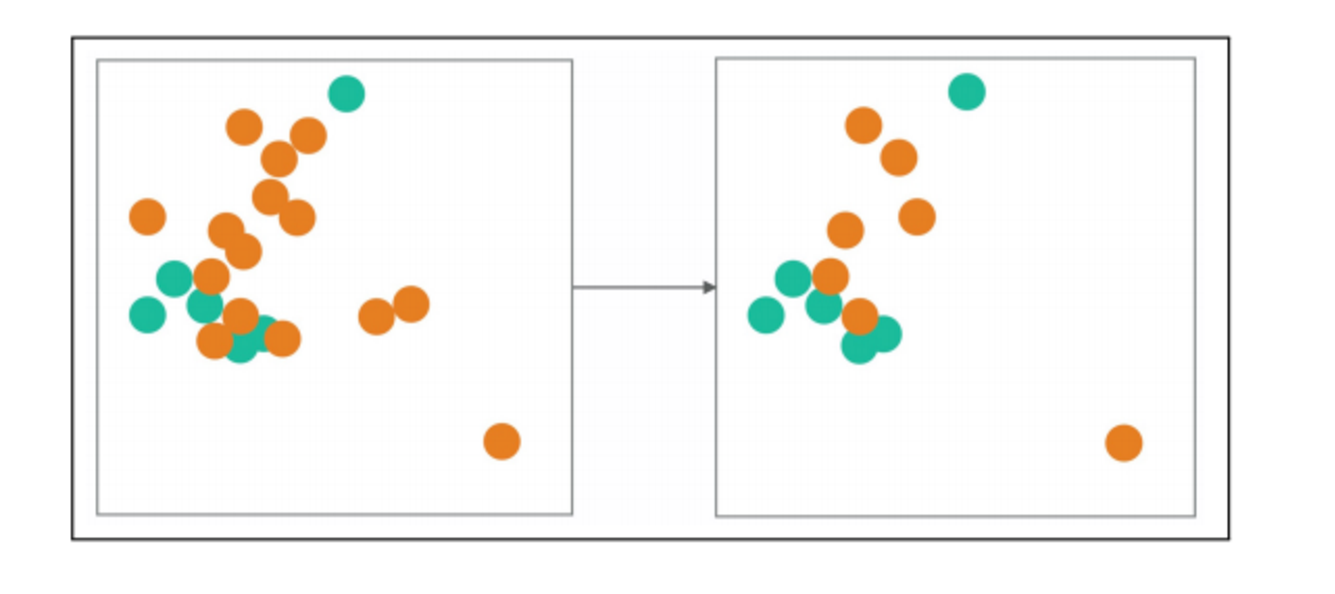
\includegraphics[width=0.45\textwidth]{figures/7.pdf}
\caption{欠采样方法示例}}
%盒子二
\parbox[h]{.5\textwidth}{\centering
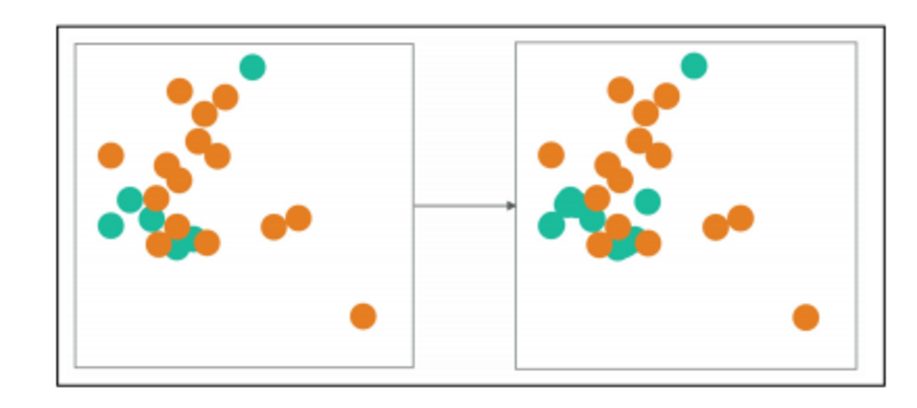
\includegraphics[width=0.45\textwidth]{figures/8.pdf}
\caption{过采样方法示例}}
\end{figure}

经过对比,本文选择了欠采样的方法。例如针对FindBugs工具,训练时在5834个检测正确的样本中随机挑选出1488个,与1488个缺陷样本一起加入训练,保证了训练数据正负样本的数量均衡。随机欠采样的方法既不会影响数据的统计特征,同时可以使正负样本的边界更为清晰。本文的测试数据采用了不同于训练数据的1000个代码样例,同样的,为了保证样本正负样本数量的均衡,每次测试时,本文从1000个样本中随机抽取正负样本各50个进行测试,测试十次得到测试的平均正确率。

\subsection{训练设置}
本次模型训练采用了TensorFlow的AdamOptimizer,AdamOptimizer实现了Adam优化算法,比起随机梯度下降的方法,Adam算法收敛速度更加迅速。训练学习率初始设置为$10^{4}$,学习率随着训练的迭代步数增加而呈阶梯状下降,每迭代100次变为原来的0.98倍。损失函数采用了交叉熵的算法,对两个概率分布$p$和$q$,通过$q$来表示$q$的交叉熵为:
$$H(p,q) = -\sum_x p(x)\log q(x)$$
通过交叉熵函数可以比较两个概率分布的差异。

针对本文提出的模型,有两个参数可能影响模型的结果:图压缩后特征向量的维度大小$d$以及压缩算法的迭代次数$T$。接下来将分别探讨两者的影响。


对于特征向量$d$,可以看出,当$d$的维度增加,网络中的参数$W_1, W_2, W_3, W_4$的维度都会相应的增加,相当于网络的每一层的神经元都会增加,网络变得更加复杂,能够拟合的函数也就越复杂,同时也有可能导致过拟合的问题。
